\documentclass[12pt]{report}
  \title{\LARGE Tools for Neural Network Simulation \\ \vspace{7mm} \large Interim Report}
  \author{ \emph{Author:} \\ Iskander Orazbekov \vspace{56 mm} \\ Imperial College London}
  \date{\today}
\usepackage{a4}
\usepackage{listings}
\usepackage{graphicx}
\usepackage{url}
\usepackage[english]{babel}
\usepackage{wrapfig}
\setlength{\parskip}{0.3cm}
\setlength{\parindent}{0cm}

\begin{document}

\maketitle

\begin{abstract}

Motivation behind the development of spiking neural networks arised from the growing interest in the area of neural 
computation and studies of brain activity in the recent years. The reason lies in the fact that SNNs incorporate time
into neuron firing computation and signify the role of interconnectedness between neurons, therefore bringing the simulation 
level closer to reality.

However, as a result of such improvement, spiking neural networks are computationally expensive to simulate, therefore, a solution 
using parallel computation was needed. NeMo, a Spiking Neural Network simulator developed at Imperial College, solves this problem 
by making use of CUDA-interfaced GPUs with high level of parallelism.

The aim of this project is to implement the Message Passing Interface for NeMo, and by doing this, improve inter-neural communication, 
to allow for better performance of parallel computations. This, in turn, will allow for bigger number of neurons within the network 
and greater level of realism brought by the simulation.

\end{abstract}

\tableofcontents

\renewcommand{\chaptername}{}

\chapter{Introduction}

Studies in the area of neuroscience have always pushed boundaries of the development of simulation tools, requiring more computational power 
for realistical models. In order to achieve a high level of realism, large-scale networks are needed, that consist of more than \begin{math}10^8\end{math} neurons 
and \begin{math}10^{12}\end{math} synapses - and manipulating that data alone comprises a challenging task.

Consequently, parallel computations are used, in order to minimize the workload given to a particular machine and to ensure that throughout
this execution all of the clusters are communicating between each other. Once implemented, this system will allow a great amount of scalability
to be put to use, enhancing the quality of simulations.

Therefore, \emph{Message Passing Interface} (MPI) improvement in the current NeMo system will allow for faster rate of computations by making use 
of parallelism. With the use of MPI, it will be possible to make full use of cluster-based implementation that will deal with the scalability by 
distributing the workload across several machines. This means that a simulation would be able to host more neurons, therefore creating a more 
realistical model of brain activity and making it more useful for the research purposes.

However, bigger number of neurons results in need for more efficient memory management, as more data would have to be stored for effective 
communication. At the same time, a mapping specific to the topology and interconnectedness of a particular network should be derived to increase
the efficiency of transmissions.

All in all, the successful implementation of the MPI communications protocol will achieve not only a greater scope of usage of NeMo simulator within
neural computing research, but also provide a good basis for future implementations and enhancements of the simulator.

\chapter{Background}

\section{Spiking Neural Networks}

An \emph{artificial neural network}(ANN) is defined as a computational model inspired by the structure and functional aspects of biological neural networks.\cite{ActFunc}
It is an adaptive system that consists of \textbf{neurons}, its basic computational units, that are connected with each other via \textbf{synapses}.
Modern neural networks are mostly used as non-linear statistical data modeling tools to find patterns between inputs and outputs.\cite{Bar-Yam2003}

\emph{Spiking neural network}(SNN) - is a third generation neural network that comprises within itself not only concepts of neuronal and synaptic states, but 
also time.\cite{Maass1997} As a result of putting emphasis on time as an acting property, a much higher level of realism is achieved in simulations,
making SNNs particularly useful for research in such areas as brain activity or neural computation.

\subsection{Artificial and Spiking Neurons}

In order to distinguish between different generations of neural networks, one would need to take into account type of neurons, as they define the type of network.

\begin{figure}[h]
\begin{center}
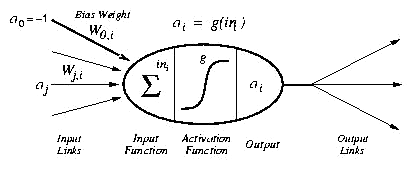
\includegraphics[scale = 0.6]{images/neuron_model.png}
\end{center}
\caption{A graphical model of a simple artificial neuron\cite{Philosophy}}
\end{figure}

Typical neural networks consist of a number of computational units, \emph{artificial neurons}. An \emph{artificial neuron} is a model of a mathematical 
function or an abstraction of biological neurons\cite{Harmon1959}, that given several inputs, derives a value based on the sum of this collection of inputs 
and built-in function, and returns this value as an output, essentially acting as an axon of a real neuron. Artificial neurons differ depending on their 
specific model, such as McCulloch-Pitts or linear-threshold function. These models define a set of properties that a particular neuron possesses, such as 
transfer (or activation) function.

\begin{figure}[h]
\begin{center}
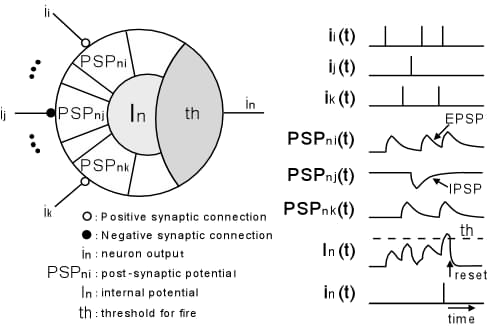
\includegraphics[scale = 0.8]{images/spiking-model.png}
\end{center}
\caption{A graphical model of a spiking neuron\cite{HidekiTanaka2009}}
\end{figure}

However, spiking neural networks are quite different in nature and, specifically, in structure of their computational units from artificial neural networks. SNNs consist of \textbf{spiking neurons} 
that aim to model the activity of real biological neurons, that is to make an abstraction which is as close as possible to the original. A \emph{spiking neuron} instead of
having set time period of emission, fires a \textbf{spike} - a very short signal that remains at its peak value for about a millisecond. Firing in spiking neurons is caused
by changes in membrane potential as well as resulting from time-based activation function. The signal is transferred to other neurons, in turn, increasing or decreasing their
membrane potential. However, since signals do not vary in value, the information is transferred via a collection of spikes, called a \emph{spike train}. Through the spike train
it is relatively easy to obtain the timing and number of spikes, therefore, these two variables hold the actual data.\cite{WulframGerstner2002} By possessing these qualities, networks 
built from spiking neurons obtain a significantly larger computational power than that of same-sized artificial neural network.\cite{Maass2003}

\subsubsection{Activation Function}

An activation function is usually an abstraction that represents the firing rate of the cell, that is dependent on the sum of inputs as well as on time.\cite{ActFunc} In spiking neural networks,
this function does not output a binary set of values, but is rather calculated through a set of differential equations that depend on the input current and, if implemented, time.

\subsubsection{Spiking Neuron Models}

Here some of the spiking (or biological) neuron models will be presented.

\begin{itemize}

\item Integrate and Fire

\emph{Integrate and Fire}(IF) model is a simple and relatively accurate representation of the actual biological neuron.
It divides the behaviour of membrane potential into two parts: long periods of \emph{integration} and short firing of \emph{spikes}. The activation function for this kind of neurons is
a time derivative of the law of capacitance, with a refactoring time added to limit the speed of firing: \begin{math}f(I) = \frac{I}{C_{m}V_{th} + t_{ref}I}\end{math}.
Therefore, the rate of firing is directly proportional to the input current.\cite{WulframGerstner2002}

However, if not modified, this model does not implement time-dependent memory. Moreover, it also lacks details in representation of biological neurons, as most of the biophysiological 
processes are simplified. For example lagging of sodium channel activation present in Hodgkin-Huxley model is absent in IF.\cite{IFModel}

\item Hodgkin and Huxley

\emph{Hodgkin and Huxley}(HH) model aims to incorporate an exhaustive description of a real biological neuron - therefore, requiring a large number of parameters to operate.
As opposed to IF, HH model uses nonlinear differential equations in its activation function to determine the membrane charasteristics and, therefore, provide the closest 
biophysical representation of a biological neuron.\cite{Hodgkin1952}

\item Izhikevich model

\emph{Izhikevich neuron model} is aiming to produce a plausible representation, close to HH, of a biological neuron, while maintaining the computational power and efficiency of an IF model.
It has several improvements over IF model, such as enhancing the activation function for the purpose of more accurate spike firing representation, which is done by introducing more 
types of spiking periods and give the implementation.\cite{Izhikevich2003}

\end{itemize}

\subsection{Synapses}

\emph{Synapses} in spiking neural networks represent dendrites in biological neural systems, making directed connections between spiking neurons. 
Therefore, synapses act as the main transmitters of spikes within the network, contributing to the connectionist approach, the main paradigm of neural networks.

\subsubsection{Synaptic Plasticity}

\emph{Synaptic plasticity} is the ability of a given synapse to change the number of receptors depending on the use.\cite{WulframGerstner2002} This represents quite an
important part of the neural network model, as it is a part of real-time alterations that occur during the actual simulation.

Spiking neural networks rely on \emph{spike timing dependent plasticity}(STDP) model for simulating plasticity, as most of information transmitted in SNNs is dependent not on 
the power of signals but rather on their timing and number. STDP rules divide the spikes occuring onto pre- and post-synaptic, determining the changes in the action potential that
they bring in. Consequently, these parameters control the extent of synaptic modification.\cite{SenSong2000}

\subsection{Topology}

Topology of a neural network is essentially its layout, that displays the connections between the neurons. Topology plays critical role, when 
the neural network is mapped onto the computational clusters, as it helps distinguish an optimal way of allocating neurons between the nodes,
and by doing this significantly increase the efficiency of communication.

\begin{figure}[h]
\begin{center}
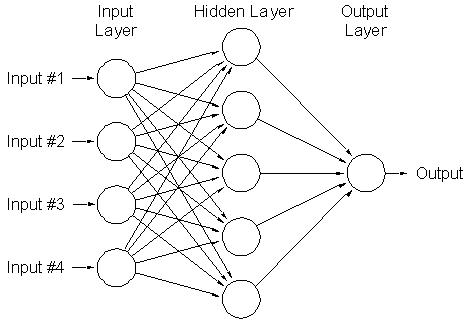
\includegraphics[scale = 0.3]{images/topology.png}
\end{center}
\caption{Topology of a feed-forward neural network\cite{Tan2006}}
\end{figure}

\section{Spiking Neural Network Simulators}

In order to give a better outlook on the field of spiking neural network simulation, this section will cover some of the state of the art solutions present to date.

\subsection{NeMo}

\emph{NeMo} is a spiking neural network simulator aimed at real-time simulation of large-scale neuron systems with the use of highly parallel GPUs.\cite{AndreasK.Fidjeland2009}
NeMo's main purpose is to produce simulations that would be particularly useful for research, therefore, main emphasis in this tool is put onto scalability and real-time aspects
of produced simulations.

NeMo is the main platform of MPI implementation for this project. The main goal is to improve inter-neural communication between computational clusters within NeMo.
At the same time, neuron mapping should be changed to ensure efficient communication during the simulation.

\subsection{Brian}

Another solution, \emph{Brian} aims for bigger flexibility and ease of use, therefore making it more suitable for teaching purposes. \cite{Goodman2008} This
particular simulator will provide a good example of an spiking neural network simulator, and as it is easy to operate, will be useful for learning main concepts
of SNN in detail.

\subsection{SpikeNET}

\emph{SpikeNET} is a spiking neural network simulator created for large-scale integrate-and-fire networks simulations.\cite{ArnaudDelorme1999} As the main aim of this project is to
achieve the highest possible number of neurons hosted and computed simultaneously, this solution requires a very high level of parallelism in order to operate.
Therefore, findings from this project would be useful later in the project, when the focus is going to be on the scale of computations.

\subsection{Blue Brain Project}

Initiated in cooperation between IBM and EPFL, the \emph{Blue Brain Project} aims to produce a virtual brain in a supercomputer, Blue Gene, provided by IBM.\cite{BlueBrain} Computational power
required for the operations is immense, however, supercomputing technology gave neuroscientists a set of tools to solve this problem. The Blue Brain simulator is
a very interesting project, and due to exceptionally difficult task of reducing workload across the stations - it will be particularly useful at the stage of MPI development.

\section{Distributed Computing}

As the main objective of the project is to enhance communication efficiency between neurons in the spiking neural network, use of distributed computing plays crucial
role in its achieving. In this context, distributed computing means parallelization of tasks across the connected system and providing efficient communication medium
between separate computational clusters.

\subsection{Parallel Computing}

\emph{Parallel computing} is a form of computation where most of calculations are carried out simultaneously.\cite{G.S.Almasi1989} In order to achieve this, large problems
are divided into smaller independent parts that are carried out by separate computational units, with feeding the results either into the main cluster or holding it for further
computations. The rise of this particular field is due to the need in high-performance computing, especially in the light of frequency scaling becoming more and more
limited because of power consumption.\cite{Kumar2002}

Due to the nature of this project, a high degree of parallelism is crucial, in order to maintain the highest possible speed of simulation - the matter is that simulation would
be split between several clusters (\emph{nodes}) which, depending on the mapping, will operate independently, after receiving the information from main node at the start.

\subsection{Message Passing Interface}

\emph{Message Passing Interface} (MPI) is a language-independent protocol which acts as a communications medium for a group of processes.\cite{mpi} MPI's main function is to provide
a solid communication channel between the processes in a highly parallelised system, thus, enhancing efficiency of this system. Message passing programs are written in Fortran and 
C, with the use of built-in functions.

Currently NeMo has an MPI implementation within it, however, it is not the most optimal one. The main idea behind parallelisation in this project is that neurons are allocated, 
using mapping algorithm, between several computational nodes, which are communicating with each other with the use of MPI. Therefore, one of the main objectives will be to 
create an MPI layer inside system, that would increase the speed of computations by enhancing quality of inter-cluster communication.

There are currently several implementations of MPI to date, so here is a brief overview of available solutions.

\subsubsection{Open MPI}

The \emph{Open MPI Project} is an open-source implementation of MPI-2 maintained by a group of academic, research and industry partners, Open MPI Team.\cite{RichardL.Graham2005} This particular 
implementation aims at compatibility and high performance on all platforms, thus, making it quite easy to install and configure. Open MPI is a useful tool that will help understand 
the underlying concepts of message passing and generally give a good background within this subject area.

\subsubsection{MPICH2}

\emph{MPICH2} is an MPI implementation from Argonne National Laboratory, that aims at high performance and extendability.\cite{W.Gropp1999} The main idea of the project is to make the simulations as
fast as possible, via enhancing the efficiency of communication, therefore, MPICH2 fits well with the aims set, by providing focus on the speed and effectiveness. Another reason to choose 
MPICH2 for this project is that this package is already installed on the lab machines, therefore, saving time for the initial setup.\cite{W.Gropp1999a}

\subsection{Cluster-based approach and Mapping}

One of the most important part of the simulation is the initial \textbf{mapping} of neurons across the hosts, as it will affect the amount of inter-cluster communication and therefore overall efficiency
of the system. \emph{Mapping} defines the layout of the resulting system and is directly affected by topology - neurons are split into several groups depending on the number of synapses connecting those.
The main idea is to keep the amount of inter-cluster communication to minimum, as it is more expensive in terms of memory and time than communication within the node.

Mapping is defined by topology and hierarchy of the system - most of implementations have a master node, accountable for adding neurons and synapses to particular clusters, however, it is
possible to have a distributed system, were all nodes are equal in resposibility and actions are taken independently.

Current implementations of cluster-based approach include:

\begin{itemize}
\item{Izhikevich's large-scale model for simulating mammalian thalamocortical systems \cite{EugeneM.Izhikevich2008}}
\item{IBM cortical simulator project\cite{DharmendraS.Modha2007}}
\item{Neuromorphic model for GPGPU cluster by Tarek M. Taha\cite{TarekM.Taha2010}}
\end{itemize}

\chapter{Project Outline}

\section{Requirements}

List of requirements, needed for the project to be running:

\begin{itemize}
\item{Access to NeMo codebase}
\item{Access to a high-performance cluster within the Department}
\item{One of the latest MPI implementations present on lab machines}
\item{Right to install libraries which this implementation is dependent on}
\item{Access to project-specific literature, covering Neural Networks, MPI and Parallel Computing}
\end{itemize}

\section{Project Plan}

In this section, a probable plan of the project is outlined.

\subsection{Part I: Introduction to Spiking Neural Networks, MPI and NeMo}

This is the initial stage of the project, during which I have made myself familiar with the SNN methodology. Most of the work was focused on research into the area of SNN simulation 
as well as parallel computing and MPI. At the same time I was reviewing the codebase of NeMo simulator, especially the current MPI implementation, in order to see how the current dependencies 
are defined, and what will be the way I integrate my own implementation into the project.

\subsection{Part II: MPI Simulation Class}

At this point I expect to have background knowledge about SNN and MPI, therefore start the development of MPI-based examples using NeMo API. After acquiring enough experience in handling
both, my intention is to start development of the actual MPI Layer for NeMo. As MPI is able to run on a single station, testing would involve writing code with MPI functions to be tested 
on a lone node and then converting it for cluster-based implementation.

\subsection{Part III: Integration of Cluster Mapping}

Once the MPI communication layer is created, the next step is to work out the mapping algorithm for pre-simulation cluster(node) setup. For now, this is going to be done in a centralized 
manner, by having a "master" node that is accountable for sending the layout (neurons and synapses) to all "worker" nodes. This implementation will require not only a fully working MPI layer,
but, probably, a set of auxiliary functions for memory management.

\subsection{Part IV: Layouts of Clusters Topology}

This is the final stage of the project - if the centralized cluster mapping is implemented, a set of different mappings could be integrated as well. These would be more aligned with distributed
paradigm, aiming for scalability and, therefore, higher level of realism of the network simulation. The implementation would include modifying existing code, writing additional communication 
functions and giving more functionality to the clusters, eliminating the "master" node.

\section{Evaluation}

The project progress is going to be evaluated based on the tests that will be run on my NeMo implementation against the "control" current one.

\subsection{Testing methods}

In order to test the resulting implementation, a testing harness would be required that will be applied to the two versions of NeMo: modified and "clean".
The tests will focus on one particular property of the simulation: number of spike arrivals per unit time, or \emph{throughput of the network}.

Throughput is going to be measured by simply counting the number of spike arrivals over a constant period of time for both implementations with following comparison.

For the purpose of the easier and clearer testing, number of free variable will be minimized, so such parameters as number of clusters, synapses and 
neurons, will be the same for both implementations, however varying for different tests. Once Part IV of the plan is reached, new implementations would also be tested alongside with the old ones, 
in order to provide a more objective overview of the changes.

\subsection{Results evaluation}

As mentioned above, the main property that define the effectiveness of the implementation is throughput.
Once the set of results for several runs of both implementations is obtained, an average is calculated and compared for different network sizes and connectivity.
The comparison ratio will, therefore, provide the evidence of a progress made.

\section{Further extensions}

This project could be extended with deeper research into the cluster-based models of SNN simulators to produce more different types of layouts that could later be used for evaluation.
Moreover, with more computational power at hand and more time, this research could be advanced into more areas, for example, closer to particular branch of brain activity studies.

\clearpage

\bibliographystyle{plain}
\bibliography{myrefs}

\end{document}
